%%%%%%%%%%%%%%%%%%%%%%%%%%%%%%%%%%%%%%%%%
%
% (c) 2019 by Jennifer Laaser
%
% This work is licensed under the Creative Commons Attribution-NonCommercial-ShareAlike 4.0 International License. To view a copy of this license, visit http://creativecommons.org/licenses/by-nc-sa/4.0/ or send a letter to Creative Commons, PO Box 1866, Mountain View, CA 94042, USA.
%
% The current source for these materials is accessible on Github: https://github.com/jlaaser/pogil-polymers
%
%%%%%%%%%%%%%%%%%%%%%%%%%%%%%%%%%%%%%%%%%

\renewcommand{\figpath}{content/polymchem/copolymers/copolym/figs}
\renewcommand{\labelbase}{copolym}

\begin{activity}{Copolymerization}

\begin{instructornotes}
	This activity introduces students to concepts related to the chemistry of copolymerization in chain-growth polymerizations
	
	After completing this activity, students will be able to:
	\begin{enumerate}
		\item \dots
	\end{enumerate}
	
	\subsection*{Activity summary:}
	\begin{itemize}
		\item \textbf{Activity type:} Learning Cycle
		\item \textbf{Content goals:} Chemistry of copolymerizations
		\item \textbf{Process goals:} %https://pogil.org/uploads/attachments/cj54b5yts006cklx4hh758htf-process-skills-official-pogil-list-2015-original.pdf
			written communication, critical thinking, information processing
		\item \textbf{Duration:} TBD
		\item \textbf{Instructor preparation required:} none beyond knowledge of relevant content
		\item \textbf{Related textbook chapters:}
			\begin{itemize}
				\item \emph{Polymer Chemistry} (Hiemenz \& Lodge): section NNN
			\end{itemize}
		%\item \textbf{Facilitation notes:}
		%	\begin{itemize}
		%		\item \dots
		%	\end{itemize}
	\end{itemize}
	
\end{instructornotes}


\begin{model}[Simulation Activity]
	\label{\labelbase:mdl:simulation}

	In copolymerizations, in which two different types of monomers are simultaneously incorporated into the same chain, the relative reactivities of the monomers can have a big impact on the polymer microstructure.
	
	Simulate a fully random copolymerization by doing the following:
	
	\begin{enumerate}
		\item Set-up the simulation:
			\begin{enumerate}
				\item Place two cups, each filled with a different color of beads, within reach of all members of your group.  Designate one color ``color A'' and the other ``color B''.
				\item Open a random number generator app on your phone and set it to generate numbers between 0 and 1 to two decimal places.  \emph{Alternatively,} obtain a sheet of random numbers from your instructor.
			\end{enumerate}
		\item Synthesize a random polymer chain:
			\begin{enumerate}
				\item Pick up a bead of either color.
				\item Generate a random number (or, read the next random number off the list).  Each student in the group should get a different random number.
				\item Add a new bead to the end of the chain according to the following rules:
					\begin{center}
					\renewcommand{\arraystretch}{1.5}
					\begin{tabular}{|c|c|c|}
						\hline
						\textbf{If the last bead was...} &  \textbf{then add an ``A'' bead if} & \textbf{or add a ``B'' bead if}\\\hline
						 an ``A'' bead & Number is $\leq 0.5$ & Number is $> 0.5$ \\
						 a ``B'' bead & Number is $\leq 0.5$ & Number is $> 0.5$ \\\hline
					\end{tabular}
					\end{center}
				\item Repeat steps (b) and (c) until your chain is 30 beads long.
			\end{enumerate}
	\end{enumerate}
	
\end{model}


\begin{ctqs}

	\question Record the sequence of the beads in your chain below.  Shade in the circles corresponding to ``A'' beads, and leave circles corresponding to ``B'' beads blank.
	
		\vspace{6pt}
		\centerline{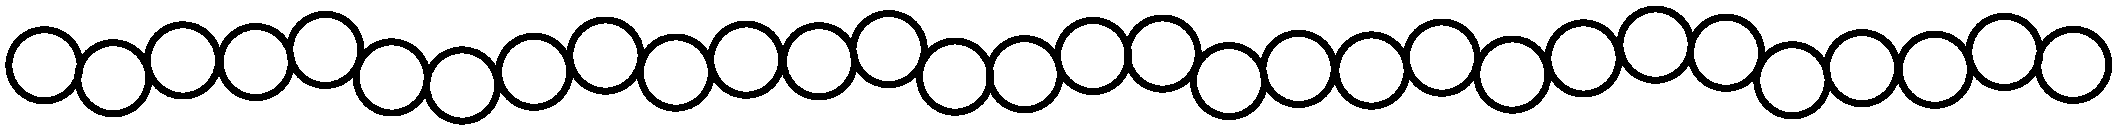
\includegraphics[width=\textwidth]{\figpath/Model1_blank.pdf}}
	
	\question Compare your polymer sequence to those of your group-mates.  What type of sequence (random, alternating, blocky) did this polymerization generally produce?
		
		\begin{solution}[1.25in]
		\end{solution}
	
	\question Repeat the process in Model 1 using the following rules:	\begin{center}
					\renewcommand{\arraystretch}{1.5}
					\begin{tabular}{|c|c|c|}
						\hline
						\textbf{If the last bead was...} &  \textbf{then add an ``A'' bead if} & \textbf{or add a ``B'' bead if}\\\hline
						 an ``A'' bead & Number is $\leq 0.2$ & Number is $> 0.2$ \\
						 a ``B'' bead & Number is $\leq 0.8$ & Number is $> 0.8$ \\\hline
					\end{tabular}
					\end{center}
	
		Then, as before, do the following:
		\begin{enumerate}
			\item Record the sequence of the beads in your chain below.  Shade in the circles corresponding to ``A'' beads, and leave circles corresponding to ``B'' beads blank.
	
		\vspace{6pt}
		\centerline{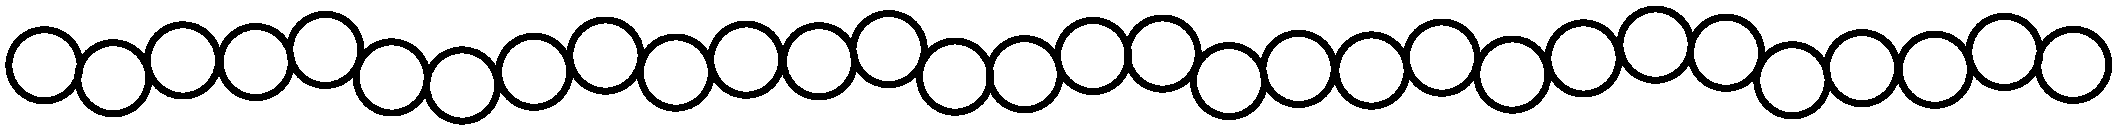
\includegraphics[width=\textwidth]{\figpath/Model1_blank.pdf}}
	
			\item Compare your polymer sequence to those of your group-mates.  What type of sequence (random, alternating, blocky) did this polymerization generally produce?
			
				\begin{solution}[1.25in]
				\end{solution}
				
		\end{enumerate}
		
		\question Repeat the process in Model 1 again, this time using the following rules:	\begin{center}
					\renewcommand{\arraystretch}{1.5}
					\begin{tabular}{|c|c|c|}
						\hline
						\textbf{If the last bead was...} &  \textbf{then add an ``A'' bead if} & \textbf{or add a ``B'' bead if}\\\hline
						 an ``A'' bead & Number is $\leq 0.8$ & Number is $> 0.8$ \\
						 a ``B'' bead & Number is $\leq 0.2$ & Number is $> 0.2$ \\\hline
					\end{tabular}
					\end{center}
	
		Then, as before, do the following:
		\begin{enumerate}
			\item Record the sequence of the beads in your chain below.  Shade in the circles corresponding to ``A'' beads, and leave circles corresponding to ``B'' beads blank.
	
		\vspace{6pt}
		\centerline{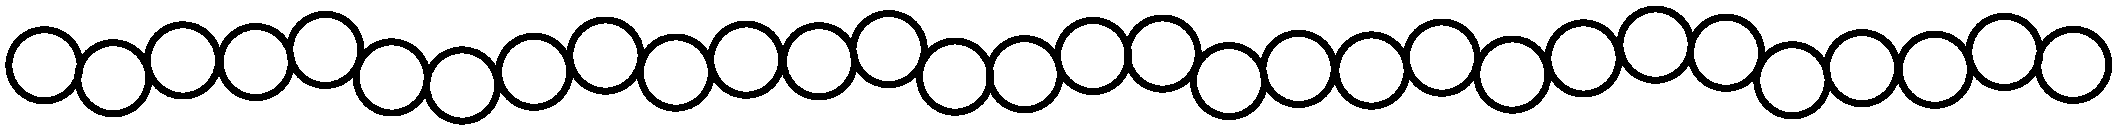
\includegraphics[width=\textwidth]{\figpath/Model1_blank.pdf}}
		
			\item Compare your polymer sequence to those of your group-mates.  What type of sequence (random, alternating, blocky) did this polymerization generally produce?
			
				\begin{solution}[1.5in]
				\end{solution}
		\end{enumerate}
		
	\question Repeat the process in Model 1 one final time using the following rules:	\begin{center}
					\renewcommand{\arraystretch}{1.5}
					\begin{tabular}{|c|c|c|}
						\hline
						\textbf{If the last bead was...} &  \textbf{then add an ``A'' bead if} & \textbf{or add a ``B'' bead if}\\\hline
						 an ``A'' bead & Number is $\leq 0.2$ & Number is $> 0.2$ \\
						 a ``B'' bead & Number is $\leq 0.2$ & Number is $> 0.2$ \\\hline
					\end{tabular}
					\end{center}
	
		Then, as before, do the following:
		\begin{enumerate}
			\item Record the sequence of the beads in your chain below.  Shade in the circles corresponding to ``A'' beads, and leave circles corresponding to ``B'' beads blank.
	
		\vspace{6pt}
		\centerline{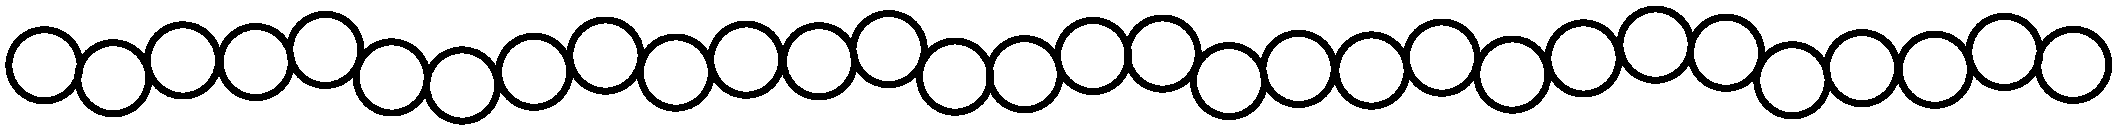
\includegraphics[width=\textwidth]{\figpath/Model1_blank.pdf}}
	
			\item Compare your polymer sequence to those of your group-mates.  What type of sequence (random, alternating, blocky) did this polymerization generally produce?
			
				\begin{solution}[1.25in]
				\end{solution}
		\end{enumerate}
		
	\question In which of the simulations did the monomers have the strongest preference for adding monomers of the \emph{same} type?
	
		\begin{solution}[0.85in]
		\end{solution}
	
	\question In which of the simulations did the monomers have the strongest preference for adding monomers of the \emph{other} type?
	
		\begin{solution}[0.85in]
		\end{solution}
	
	\question In which of the simulations did the monomers not ``care'' what type of monomer came before them?
	
		\begin{solution}[0.85in]
		\end{solution}
	
	\question In 2-3 complete sentences, describe how the preference of the monomers for adding monomers of the same or different types influences the type of sequence obtained in the copolymerization.
	
		\begin{solution}[2in]
		\end{solution}
\end{ctqs}

\begin{model}[Kinetics of Copolymerization]

	In a copolymerization reaction of monomers $M_1$ and $M_2$, there are four possible propagation steps, each with their own rate constant.  These propagation steps are:
	
	\begin{center}
		\renewcommand{\arraystretch}{1.8}
		\begin{tabular}{|c|c|}
			\hline
			\textbf{Reaction} & \textbf{Rate Law} \\\hline
			$-M_1^\bullet + M_1 \xlongrightarrow{k_{11}} -M_1M_1^\bullet$ & $R_{p,11} = k_{11}[-M_1^\bullet][M_1]$ \\\hline
			$-M_1^\bullet + M_2 \xlongrightarrow{k_{12}} -M_1M_2^\bullet$ & $R_{p,12} = k_{12}[-M_1^\bullet][M_2]$ \\\hline
			$-M_2^\bullet + M_1 \xlongrightarrow{k_{21}} -M_2M_1^\bullet$ & $R_{p,21} = k_{21}[-M_2^\bullet][M_1]$ \\\hline
			$-M_2^\bullet + M_2 \xlongrightarrow{k_{22}} -M_2M_2^\bullet$ & $R_{p,22} = k_{22}[-M_2^\bullet][M_2]$ \\\hline
		\end{tabular}
	\end{center}

\end{model}

\begin{ctqs}

	\question Suppose a propagating chain has an $M_1^\bullet$ radical on its active end.  If $R_{p,11}>R_{p,12}$, will the chain be more likely to add an $M_1$ or an $M_2$ monomer next?
	
		\begin{solution}[0.5in]
		\end{solution}
	
	\question Explain, in 1-2 complete sentences, how the ratio $R_{p,11}/R_{p,22}$ should be related to the relative probability for a chain ending in $M_1^\bullet$ to add another monomer of type $M_1$.
	
		\begin{solution}[1in]
		\end{solution}
	
	\question The rates investigated in the previous question depend on the concentrations of the monomers.  If both monomers are present in equal concentration (i.e. $[M_1]=[M_2]$), what is the value of this ratio in terms of the rate constants $k_{11}$ and $k_{22}$?
	
		\begin{solution}[1in]
		\end{solution}
	
	\question Explain, in 1-2 complete sentences, why the ratio $k_{11}/k_{12}$ is related to the relative \emph{preference} for a chain ending in $M_1^\bullet$ to add another monomer of type $M_1$.
	
		\begin{solution}[1.5in]
		\end{solution}
	
\end{ctqs}

\begin{infobox}

	We typically  describe the relative reactivities of monomers 1 and 2 using \emph{reactivity ratios} $r_1$ and $r_2$, which are defined as
	\begin{align*}
		r_1 = \frac{k_{11}}{k_{12}} && r_2 = \frac{k_{22}}{k_{21}}
	\end{align*}

\end{infobox}

\begin{ctqs}

	\question In Model 1, the rates of each monomer addition were essentially the probabilities for adding each type of monomer.  Using this information, determine the reactivity ratios for each of the copolymerizations you carried out in Model \ref{\labelbase:mdl:simulation}:
	
		\begin{center}
		\renewcommand{\arraystretch}{2.5}
		\begin{tabular}{|c|c|c|}
			\hline
			\textbf{Simulation} & ~~~~~~$r_1$~~~~~~ & ~~~~~~$r_2$~~~~~~ \\\hline
			\textbf{Model 1/CTQ 1} & & \\\hline
			\textbf{CTQ 3} & & \\\hline
			\textbf{CTQ 4} & & \\\hline
			\textbf{CTQ 5} & & \\\hline
		\end{tabular}
		\end{center}

	\question Based on what you learned in Model \ref{\labelbase:mdl:simulation}, what type of sequence (random, alternating, blocky, etc.) do you expect when...
	
		\begin{enumerate}
			\item $r_1 = 1$ and $r_2$ = 1?
			
				\begin{solution}[0.25in]
				\end{solution}
			
			\item $r_1 = \frac{1}{r_2} \neq 1$?
			
				\begin{solution}[0.25in]
				\end{solution}
			
			\item $r_1 < 1$ and $r_2 < 1$?
			
				\begin{solution}[0.25in]
				\end{solution}
			
			\item $r_1 > 1$ and $r_2 > 1$?
			
				\begin{solution}[0.25in]
				\end{solution}
		\end{enumerate}

\end{ctqs}

\begin{model}[Feed Ratios]
	\label{\labelbase:mdl:feedratios}
	
	Often, the most important thing for us to know is how the composition of the polymer being formed is related to the composition of the monomer mixture.
	
	Working through the kinetics, it is possible to show that if the fraction of unreacted monomers that are type $M_1$ is $f_1$, then the fraction of monomers that are incorporated into the polymer chain that are type $M_1$, $F_1$, is
	\begin{equation*}
		F_1 = \frac{r_1f_1^2 + f_1f_2}{r_1f_1^2+2f_1f_2 + r_2f_2^2}
	\end{equation*}
	where $f_2 = 1-f_1$.

\end{model}

\begin{ctqs}
	\question A plot of $F_1$ vs. $f_1$ is shown below for $r_1 = 4$, $r_2=0.25$: \label{\labelbase:ctq:feedratplot}
	
		\centerline{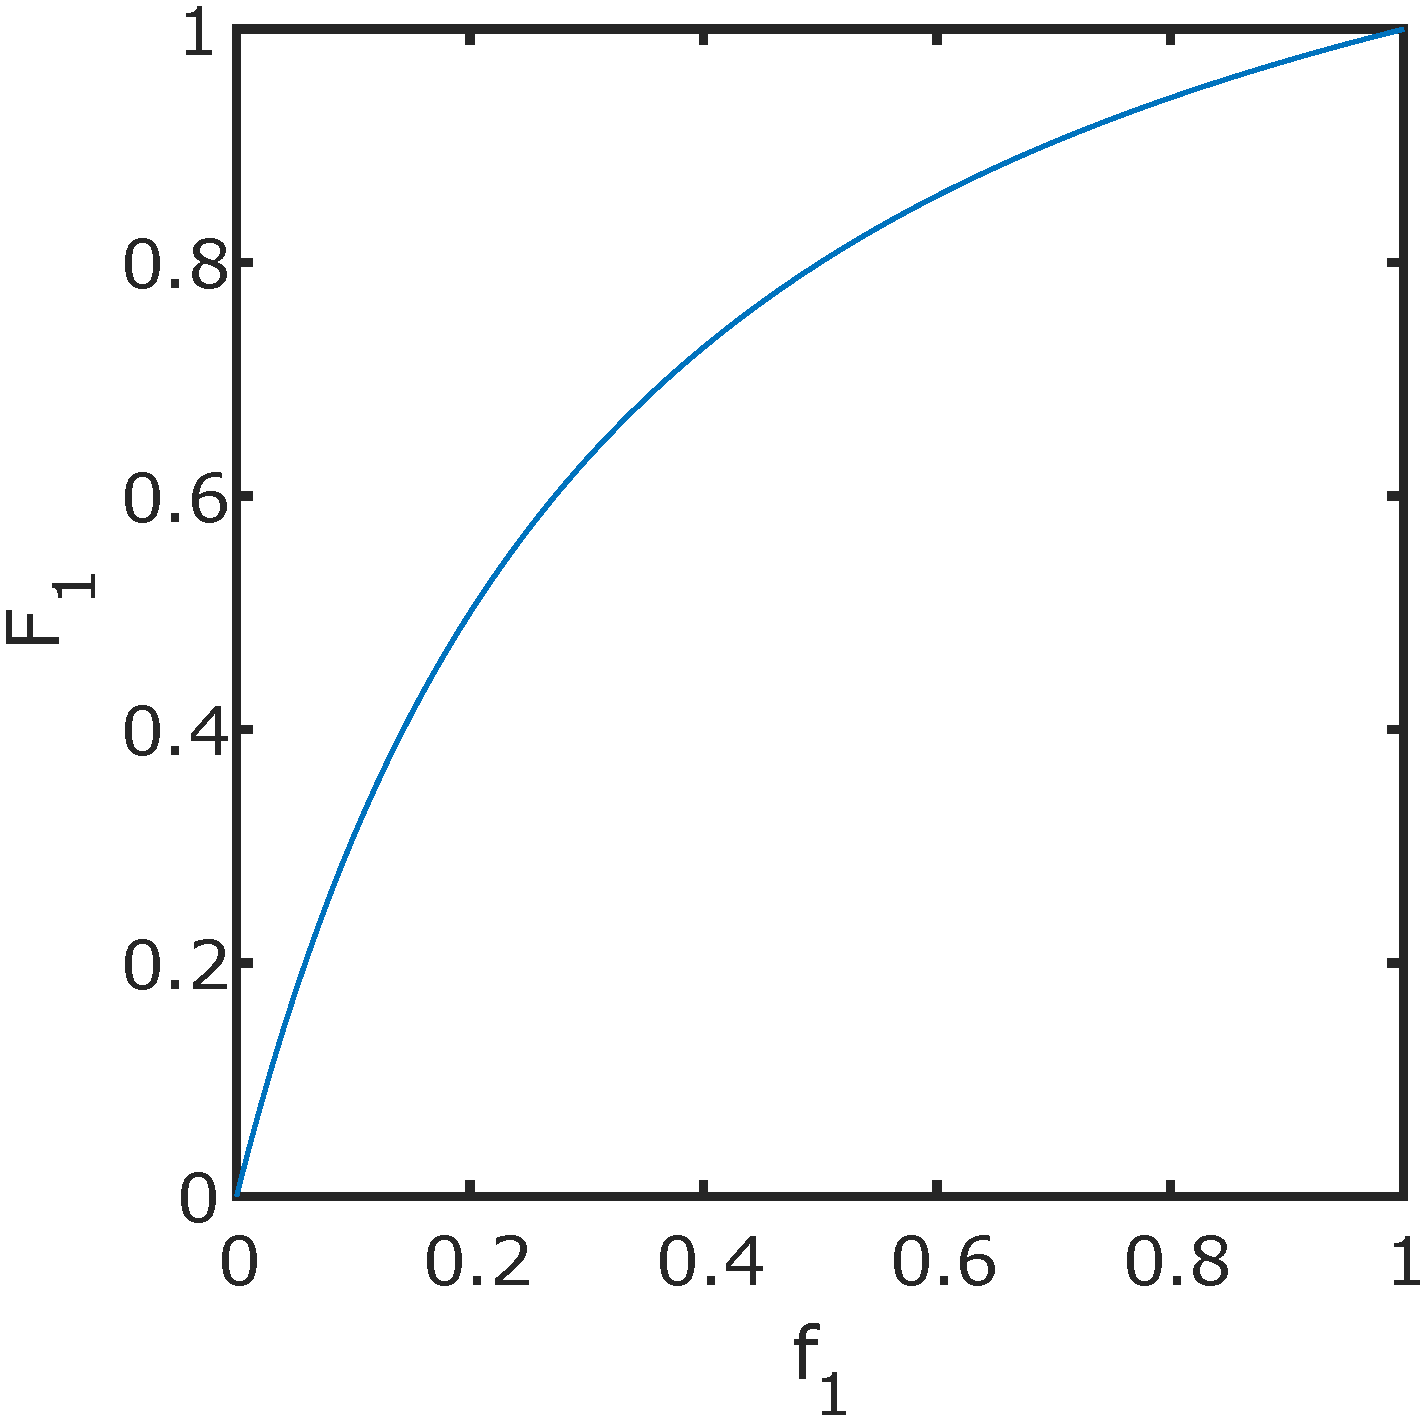
\includegraphics[width=0.4\textwidth]{\figpath/Model3_r1-4_r2-0,25.pdf}}
	
		\begin{enumerate}
			\item Qualitatively, why should $r_1 = 4$, $r_2=0.25$ generate this shape of plot?  Briefly explain your reasoning in 1-2 complete sentences.
				
				\begin{solution}[1.5in]
				\end{solution}
			
			
			\item Based on this plot, if the monomer mixture contains exactly 50\% $M_1$ monomers and 50\% $M_2$ monomers, what will the composition of the polymer being formed be? 
			
				\emph{(Hint: start by figuring out what $f_1$ is!)}
				
				\begin{solution}[0.5in]
				\end{solution}
			
			\item As the reaction goes, what will happen to the concentration of monomer $M_1$ left in solution?
				
				\begin{solution}[1in]
				\end{solution}
			
			\item Predict how the values of $f_1$ and $F_1$ are likely to change over time in this reaction.
				
				\begin{solution}[1in]
				\end{solution}
			
			\item Briefly describe the overall type of sequence you expect to generate in polymers formed in this reaction.
				
				\begin{solution}[1in]
				\end{solution}
		\end{enumerate}
\end{ctqs}


\begin{exercises}

	\exercise Make plots analogous to the plot in CTQ \ref{\labelbase:ctq:feedratplot} for (a) $r_1=1$, $r_2=1$, (b) $r_1=0.1$, $r_2=10$, (c) and $r_1=0.33$, $r_2 = 0.67$.  For each plot, explain why it has the shape that it does, and predict how the composition of the polymer would change with time for a polymerization that starts at $f_1=0.5$.
	
\end{exercises}


%\begin{problems}
%
%	\problem First exercise
%	\problem Second exercise
%	
%\end{problems}


	
\end{activity}